\documentclass[12pt,a4paper]{article}

% Essential packages
\usepackage[margin=1in]{geometry}
\usepackage{graphicx}
\usepackage{amsmath}
\usepackage{amssymb}
\usepackage{listings}
\usepackage[table]{xcolor}
\usepackage{hyperref}
\usepackage{titling}
\usepackage{float}
\usepackage{enumitem}
\usepackage{fancyhdr}
\usepackage{placeins}

% Additional packages for beautification
\usepackage[skins,breakable]{tcolorbox}
\usepackage{fontspec}
\usepackage{booktabs}
\usepackage{mdframed}
\usepackage{caption}
\usepackage{soul}
\usepackage{verbatim}

\usepackage{array}
\setlength{\tabcolsep}{6pt}

% Color definitions
\definecolor{titleblue}{RGB}{0,76,151}
\definecolor{myblue}{RGB}{25,25,112}
\definecolor{lightbluegray}{RGB}{220,230,245}  
\definecolor{mygreen}{RGB}{0,128,0}

% Custom tcolorbox styles
\tcbset{
    mybox/.style={
        enhanced,
        colback=myblue!3,
        colframe=myblue,
        arc=2mm,
        boxrule=0.8pt
    }
}

\newtcolorbox{mytitledbox}[1]{
    enhanced,
    colback=myblue!3,
    colframe=titleblue!50,
    arc=2mm,
    boxrule=1.1pt,
    title={\textcolor{white}{\textbf{#1}}},
    coltitle=white,
    fonttitle=\bfseries,
    colbacktitle=titleblue!50
}

\newtcolorbox{solutionbox}{
    enhanced,
    colback=lightbluegray!80,  
    colframe=titleblue!50,     
    arc=1.5mm,                
    boxrule=0.15pt,            
    top=2mm,                 
    bottom=2mm,
    before=\vspace{2mm},       % Space before box
    after=\vspace{2mm},        % Space after box
    breakable                  % For long solutions
}

% Header and footer setup
\pagestyle{fancy}
\fancyhf{}
\renewcommand{\headrulewidth}{0.8pt}
\renewcommand{\footrulewidth}{0.4pt}
\fancyhead[L]{\textsf{\textcolor{myblue}{Microprocessors Laboratory}}}
\fancyhead[R]{\textsf{\textcolor{myblue}{Lab 2 Report}}}
\fancyfoot[C]{\thepage}
\setlength{\headheight}{14.5pt}
\addtolength{\topmargin}{-2.5pt}

% Custom section styling
\usepackage{titlesec}
\titleformat{\section}
  {\normalfont\Large\bfseries\color{myblue}}
  {\thesection}{1em}{}[\titlerule]
\titleformat{\subsection}
  {\normalfont\large\bfseries\color{myblue}}
  {\thesubsection}{1em}{}
\titleformat{\subsubsection}
  {\normalfont\normalsize\bfseries\color{myblue}}
  {\thesubsubsection}{1em}{}


\title{
    \vspace*{2cm}
    \Huge\textbf{\textsf{Microprocessors Laboratory Report}}\\
    \vspace{0.4cm}
    \Large\textsf{Lab 2: Interrupt-Driven LED Control with UART Communication}
    \vspace{1cm}
    \rule{\textwidth}{1pt}
}

\author{
    \Large\begin{tabular}{rl}
        \textbf{Fraidakis Ioannis}\\
    \end{tabular}
}
\date{\Large\textsf{May 2025}}

% Listing style for code
\lstdefinestyle{mystyle}{
    backgroundcolor=\color{mygray},
    commentstyle=\color{mygreen},
    keywordstyle=\color{blue},
    numberstyle=\tiny\color{gray},
    stringstyle=\color{purple},
    basicstyle=\ttfamily\small,
    breakatwhitespace=false,
    breaklines=true,
    captionpos=b,
    keepspaces=true,
    numbers=left,
    numbersep=5pt,
    showspaces=false,
    showstringspaces=false,
    showtabs=false,
    tabsize=2,
    frame=single,
    framesep=5pt,
    framerule=0.5pt,
    framexleftmargin=6pt,
    framexrightmargin=6pt,
    framextopmargin=4pt,
    framexbottommargin=4pt,
}
\lstset{style=mystyle}

\begin{document}
\maketitle

\section{Introduction}

\begin{tcolorbox}[mybox]
This laboratory exercise focuses on developing an interrupt-driven LED control system that demonstrates fundamental microcontroller programming concepts. The project implements a user interface combining UART communication with physical button input to control an LED in various patterns.

The system processes numerical input where even digits trigger blinking behavior and odd digits toggle the LED state. A key feature is the ability to lock/unlock the LED via button press, preventing state changes during digit processing. 
The following sections detail the system architecture, implementation approach, testing methodology, and key insights gained from the development process.
\end{tcolorbox}

\section{System Overview}

\subsection{Hardware Components}
The system interacts with the following hardware components:


\begin{tcolorbox}[mybox]
\begin{itemize}[label=\textcolor{myblue}{$\bullet$}, itemsep=1.5mm]
    \item \textbf{LED:} Connected to GPIO pin \texttt{PA\_5}, used for visual feedback.
    \item \textbf{Button:} Connected to GPIO pin \texttt{PC\_13}, used for user interaction (locking/unlocking the LED). It is configured with an internal pull-up resistor and triggers an interrupt on a rising edge.
\end{itemize}
\end{tcolorbox}

\subsection{Software Architecture}

\subsubsection{Key Data Structures}

\begin{mytitledbox}{Data Structures}
\begin{itemize}[label=\textcolor{myblue}{$\circ$}, itemsep=1.5mm]
    \item \textbf{System (\texttt{sys\_state}):} A global \texttt{volatile struct} named \texttt{sys\_state} centralizes all dynamic data and operational flags. The \texttt{volatile} keyword ensures that the compiler correctly handles accesses to this structure, as it can be modified by Interrupt Service Routines (ISRs).

    \item \textbf{UART Receive Queue (\texttt{rx\_queue}):} A queue of type \texttt{Queue} (defined in \texttt{queue.h}) is used to buffer characters received via UART. This decouples the UART ISR from the main processing loop.
\end{itemize}
\end{mytitledbox}

\vspace{2mm}

\subsubsection{State Machine}
The system operates using a state machine with two main states:

\begin{tcolorbox}[mybox]
\begin{itemize}[label=\textcolor{myblue}{$\blacktriangleright$}, itemsep=1.5mm]
    \item \textbf{STATE\_IDLE}: The system is waiting for user input.
    \item \textbf{STATE\_PROCESSING}: The system is processing a sequence of digits.
\end{itemize}
\end{tcolorbox}

\vspace{2mm}

\begin{center}
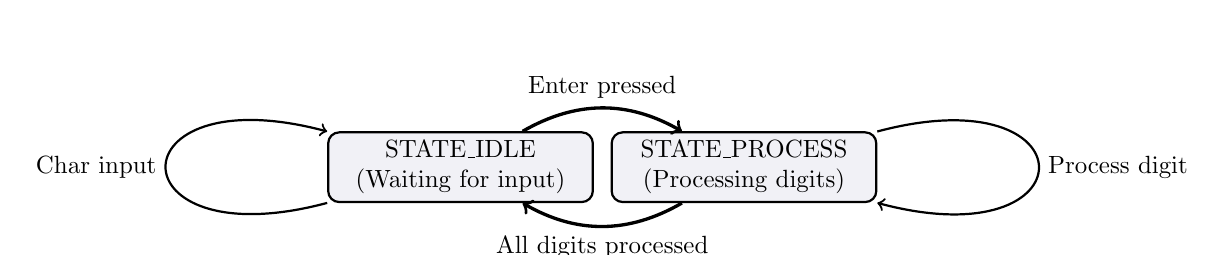
\begin{tikzpicture}[node distance=4cm, auto, thick, scale=0.9, transform shape]
    % Nodes
    \node[draw, rounded corners, fill=myblue!6, text width=3.5cm, align=center] (idle) {STATE\_IDLE\\(Waiting for input)};
    \node[draw, rounded corners, fill=myblue!6, text width=3.5cm, align=center, right of=idle] (proc) {STATE\_PROCESS\\(Processing digits)};
    
    % Edges
    \draw[->, very thick] (idle) to[bend left] node[above] {Enter pressed} (proc);
    \draw[->, very thick] (proc) to[bend left] node[below] {All digits processed} (idle);
    \draw[->, thick] (idle) to[loop left] node[left] {Char input} ();
    \draw[->, thick] (proc) to[loop right] node[right] {Process digit} ();
\end{tikzpicture}
\end{center}

\vspace{2mm}

\subsubsection{Interrupt Service Routines}
Three main interrupt handlers manage system events:

\begin{tcolorbox}[mybox]
\begin{itemize}[label=\textcolor{myblue}{$\blacktriangleright$}, itemsep=1.5mm]
    \item \textbf{timer\_callback()}: Manages timing for LED blinking and digit processing.
    \item \textbf{button\_press\_callback()}: Handles button press, toggling LED lock state.
    \item \textbf{uart\_rx\_callback()}: Adds incoming UART characters to a receive queue.
\end{itemize}
\end{tcolorbox}

\section{Testing}

\begin{mytitledbox}{Test Scenarios }
\begin{tabular}{@{}p{0.25\textwidth}p{0.35\textwidth}p{0.35\textwidth}@{}}
\toprule[1.5pt]
\textbf{\textcolor{myblue}{Action}} & \textbf{\textcolor{myblue}{Input/Event}} & \textbf{\textcolor{myblue}{Expected Outcome}} \\
\midrule[0.8pt]
Basic Blink    & UART: "24" & LED blinks for digit 2, then for digit 4. \\
\rowcolor{lightbluegray!55} Basic Toggle   & UART: "13" & LED toggles for digit 1, then for digit 3. \\
Mixed Sequence & UART: "123" & LED toggles, then blinks, then toggles. \\
\rowcolor{lightbluegray!55} Repeat Sequenc & UART: "28-" & LED blinks for 2, then for 8, then repeats. \\
LED Lock       & Press Button       & UART shows "LED Status: LOCKED". \\
\rowcolor{lightbluegray!55} Empty Input    & UART: Enter        & "No input. Enter new number:" prompt. \\
Hyphen Only    & UART: "- - -" & "No valid digits to process." prompt. \\
\rowcolor{lightbluegray!55} Extra Hyphens & UART: "1-2-3" and "8-1-" & Processes as "123" and "81" (repeat). \\
Non-Digit Chars & UART: "1a2b-c3d" & Processes as "123". \\
\rowcolor{lightbluegray!55} Backspace      & UART: "123" + Backspace & Input becomes "12", terminal cursor moves back. \\
Buffer Full    & UART: (33 digits)  & Processes first 32 digits. \\
\rowcolor{lightbluegray!55} Ctrl+C         & Press Ctrl+C       & Terminal clears, prompt reappears. \\
Ctrl+X         & Press Ctrl+X       & Program termination message, LED off. \\

\bottomrule[1.5pt]
\end{tabular}
\end{mytitledbox}
\captionof{table}{Example Test Scenarios and Expected Outcomes}

\vspace{1cm}

\begin{mytitledbox}{Validation Steps}
\begin{itemize}[label=\textcolor{myblue}{$\checkmark$}, itemsep=1.5mm]
    \item Send various digit sequences and observe LED behavior and UART output.
    \item Verify correct timing for blinking and digit processing.
    \item Press the button at different times (idle, during processing) and verify lock/unlock functionality.
    \item Test boundary conditions like empty input, full buffer, and special characters.
\end{itemize}
\end{mytitledbox}

\subsection{Challenges and Solutions}
% During implementation, several challenges were encountered:

\begin{mytitledbox}{Challenges and Solutions}
\begin{enumerate}[label=\textcolor{myblue}{\textbf{\arabic*.}}, itemsep=1.5mm]    

    \item \textbf{Keeping ISRs Short and Simple:} 
    Interrupts can occur at any time and potentially interrupt critical operations. Long or complex code execution within ISRs can lead to system instability, missed interrupts, and timing issues. This was particularly concerning for our system with multiple interrupt sources (timer, button, UART).
    
    \begin{solutionbox}
    \textit{Solution:} We implemented a flag-based approach where ISRs would only update relevant status flags in the global \texttt{sys\_state} structure rather than performing complex operations. For example, the button ISR simply sets \texttt{sys\_state.button\_event = 1} and the timer ISR sets \texttt{sys\_state.digit\_ready = 1} when appropriate. The main function then checks these flags during each iteration and performs the necessary processing. This keeps ISRs short and responsive while offloading complex logic to the main execution thread.
    \end{solutionbox}

    \item \textbf{Handling New Input During Processing:} 
    New UART inputs during digit sequence processing could interfere with ongoing operations.
    
    \begin{solutionbox}
    \textit{Solution:} Adopted a two-buffer strategy with reception buffer and separate processing buffer that isolates active processing from new inputs.
    \end{solutionbox}

\item \textbf{Button Press Detection:} We encountered a critical issue with our button interrupts. Since our button is active-low (connecting to ground when pressed), we configured it with pull-up resistors, making the pin naturally HIGH when not pressed and LOW when pressed. The problem was two-fold:

    1) The interrupt handler contained a condition checking \verb|if(p->IDR&(1<<IRQ_pin_index))| that would only execute the callback when the pin was detected as HIGH
    
    2) Even when using falling edge detection (which would trigger on button press), the callback would never execute because immediately after the falling edge, the pin would be LOW, failing the HIGH-checking condition

    \begin{solutionbox}
    \textit{Solution:} We modified the GPIO driver to execute the callback regardless of pin state after an interrupt is triggered. This allowed us to properly use falling edge detection with pull-up resistors, making the system respond when the button is actually pressed (transitioning HIGH→LOW). This approach—using pull-up resistors with falling edge detection—is actually the preferred configuration for button interfaces in embedded systems (better noise immunity and responsiveness, as actions now triggered immediately on button press rather than release).
    % Additionally, we implemented a software debouncing mechanism using a timer to prevent multiple interrupts from a single button press. After an initial interrupt, further button interrupts were ignored for a short period (approximately 50ms) to allow the mechanical contacts to settle.
    \end{solutionbox}
    
    
\end{enumerate}
\end{mytitledbox}

% \section{Conclusion}

% \begin{tcolorbox}[mybox]
% \end{tcolorbox}

% \section*{References}
% \begin{itemize}[label=\textcolor{myblue}{$\triangleright$}]
%     \item Microcontroller Datasheet (STM NUCLEO-F411RE)
% \end{itemize}

\end{document}